\section{Experiments}
In this part we compare MLE with GP and Naive method. 
\subsection{Data}
\subsubsection{Simulations}
For each experiment a diploid population is created and evolved as follows. 
\paragraph{I. Creating initial founder lines}
First using msms prgram, we created a population for $F$ founding haplotypes with parameters \texttt{\$./msms <F> 1 -t <4μLNe> -r <4Ne(L − 1)r> <L>} where $F=200$ is number of founder lines, 
$L=10^5$, $\theta=4\mu LNe=17$ and $\rho=4Ne(L-1)r=4$.  (assuming $Ne=1000$, $r=10^{-8}$ and $\mu=4.25\times 10^{-8}$).  
\paragraph{II. Creating initial diploid population} 
To mimic the real E\&R experiment for diploid organisms, first initial haplotypes cloned to create $F$ diploid homozygotes. Then each diploid is cloned $N/F$ times to yield $N$ diploid homozygote organisms.
\paragraph{III. Forward Simulation}
Given initial diploid population, position of the site under selection, selection strength $s$, number of replicates $R=3$, recombination rate $r=10^{-8}$ and sampling times $\Tc=\{10,20,30,40,50\}$ simuPop is used to perform forward simulation and compute allele frequencies for all of the $R$.

\subsubsection{Real}

\subsection{Likelihood Ratio Test}
Using the MLE (and other) estimates of $s$ it is desirable to perform a secondary task such as \emph{testing for selection} or \emph{locating the site under selection}. Likelihood ratio test (LRT) statistics for time series \cite{feder2014} have shown to be predictors for differentiating neutral and natural selection evolution cases. For a single locus model, the likelihood ratio test statistics $\Lambda(s*)$ is defined
\beq \label{eq:lrt}
\Lambda(s^*) = \log \left(\frac{\Lc(\bfX|s=s*)}{\Lc(\bfX|s=0)}\right)
\eeq
where $s^*$ is the optimal solution for the maximum-likelihood procedure. For the Gaussian process and Gaussian model the likelihood $\Lc_{GP}$ and $\Lc_G$ are well defined and \eqref{eq:lrt} can be easily evaluated. The likelihood of the Naive method for estimating based on $x_t$ is 
\beq
\Lc_N(s|x_t,x_0)=x_t-\sigma(st/2 -c)
\eeq

In addition to LRT, the value of $s^*$ itself can be regarded as a signal for detecting selection. In other words, modifying the LRT to
\beq
\Theta=s^*\Lambda(s^*)
\eeq
will take into account of two different objectives, 1)model discrepancy from neutral model 2)strength of selection under non-neutral model. In the  results we show that the modified-LRT makes more accurate predictions.

\subsection{Results}
In this part we compare the computational and predictive performance of the proposed method in detecting selection, locating selection in the genome, and estimating strength of selection with Gaussian process and the outlined naive method.

\subsubsection{Detecting Selection}
Detecting selection in the whole genome is a non-trivial task in real world and can be regarded as a application for the proposed algorithm. To provide a fair and unbiased comparison, we computed the test statistic for 1000 simulations and computed Receiver Operative Characteristic curve and Area Under Curve (AUC) for each method.
\begin{figure}[H]
  \centering
    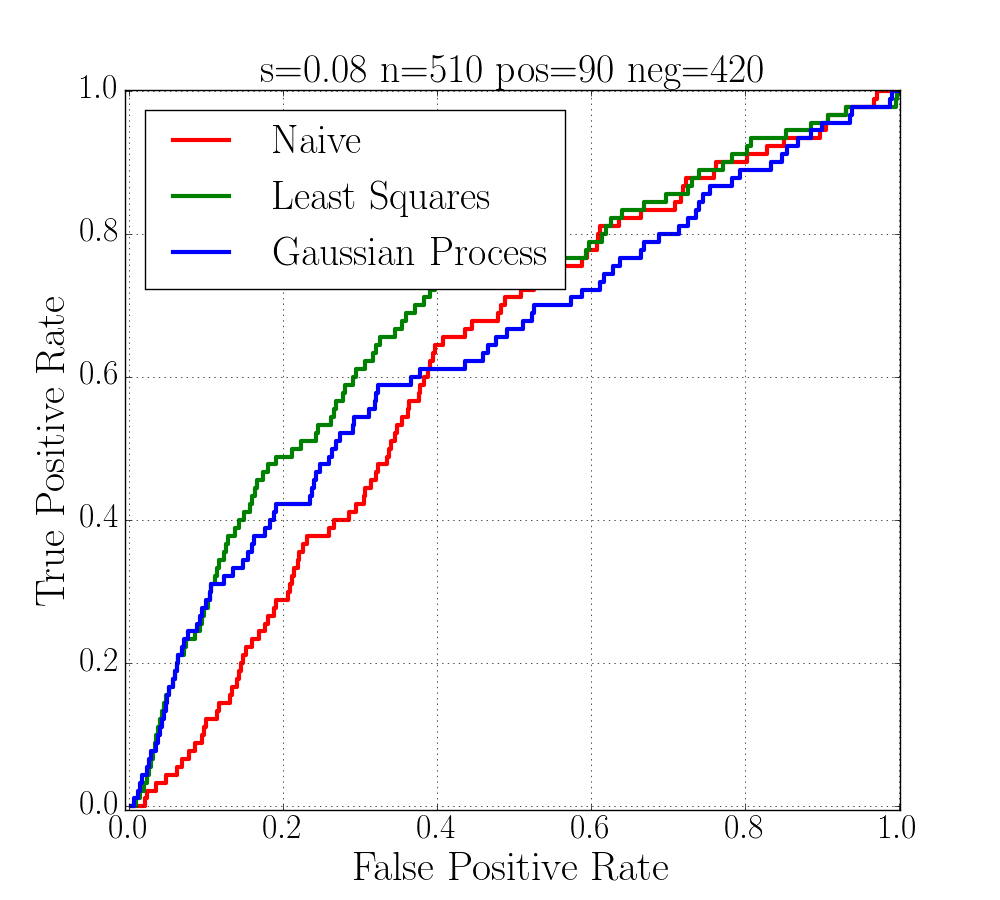
\includegraphics[width=\textwidth]{roc008}
  \caption{Rank}
  \label{fig:Fig3}
\end{figure}

\begin{figure}[H]
  \centering
    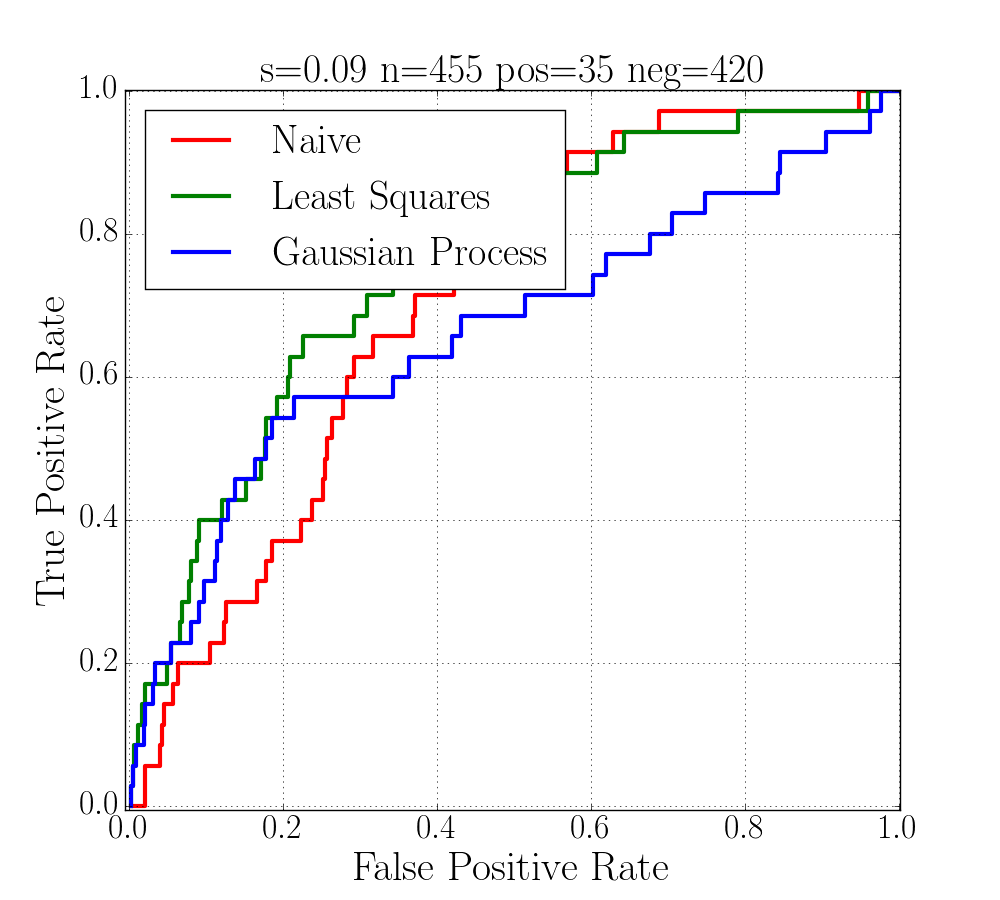
\includegraphics[width=\textwidth]{roc009}
  \caption{Rank}
  \label{fig:Fig3}
\end{figure}

\begin{figure}[H]
  \centering
    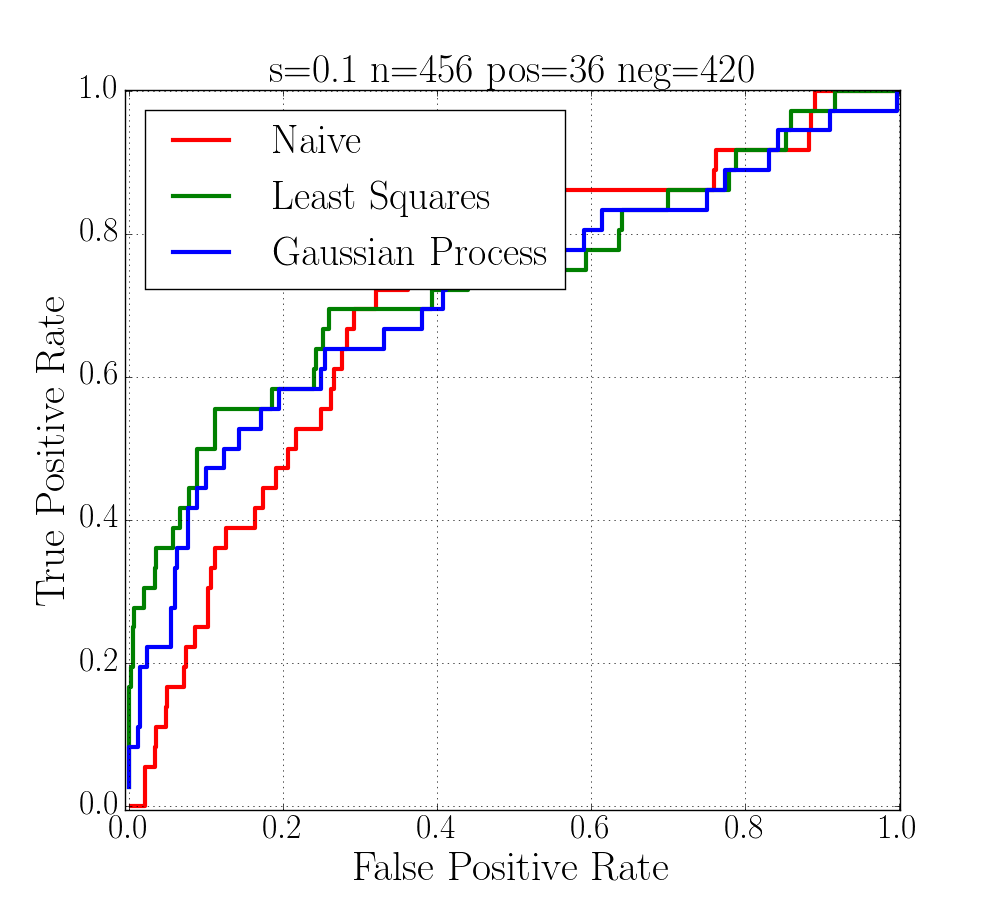
\includegraphics[width=\textwidth]{roc01}
  \caption{Rank}
  \label{fig:Fig3}
\end{figure}


\subsubsection{Finding Site Under Selection}
\paragraph{Distance}
\begin{figure}[H]
  \centering
    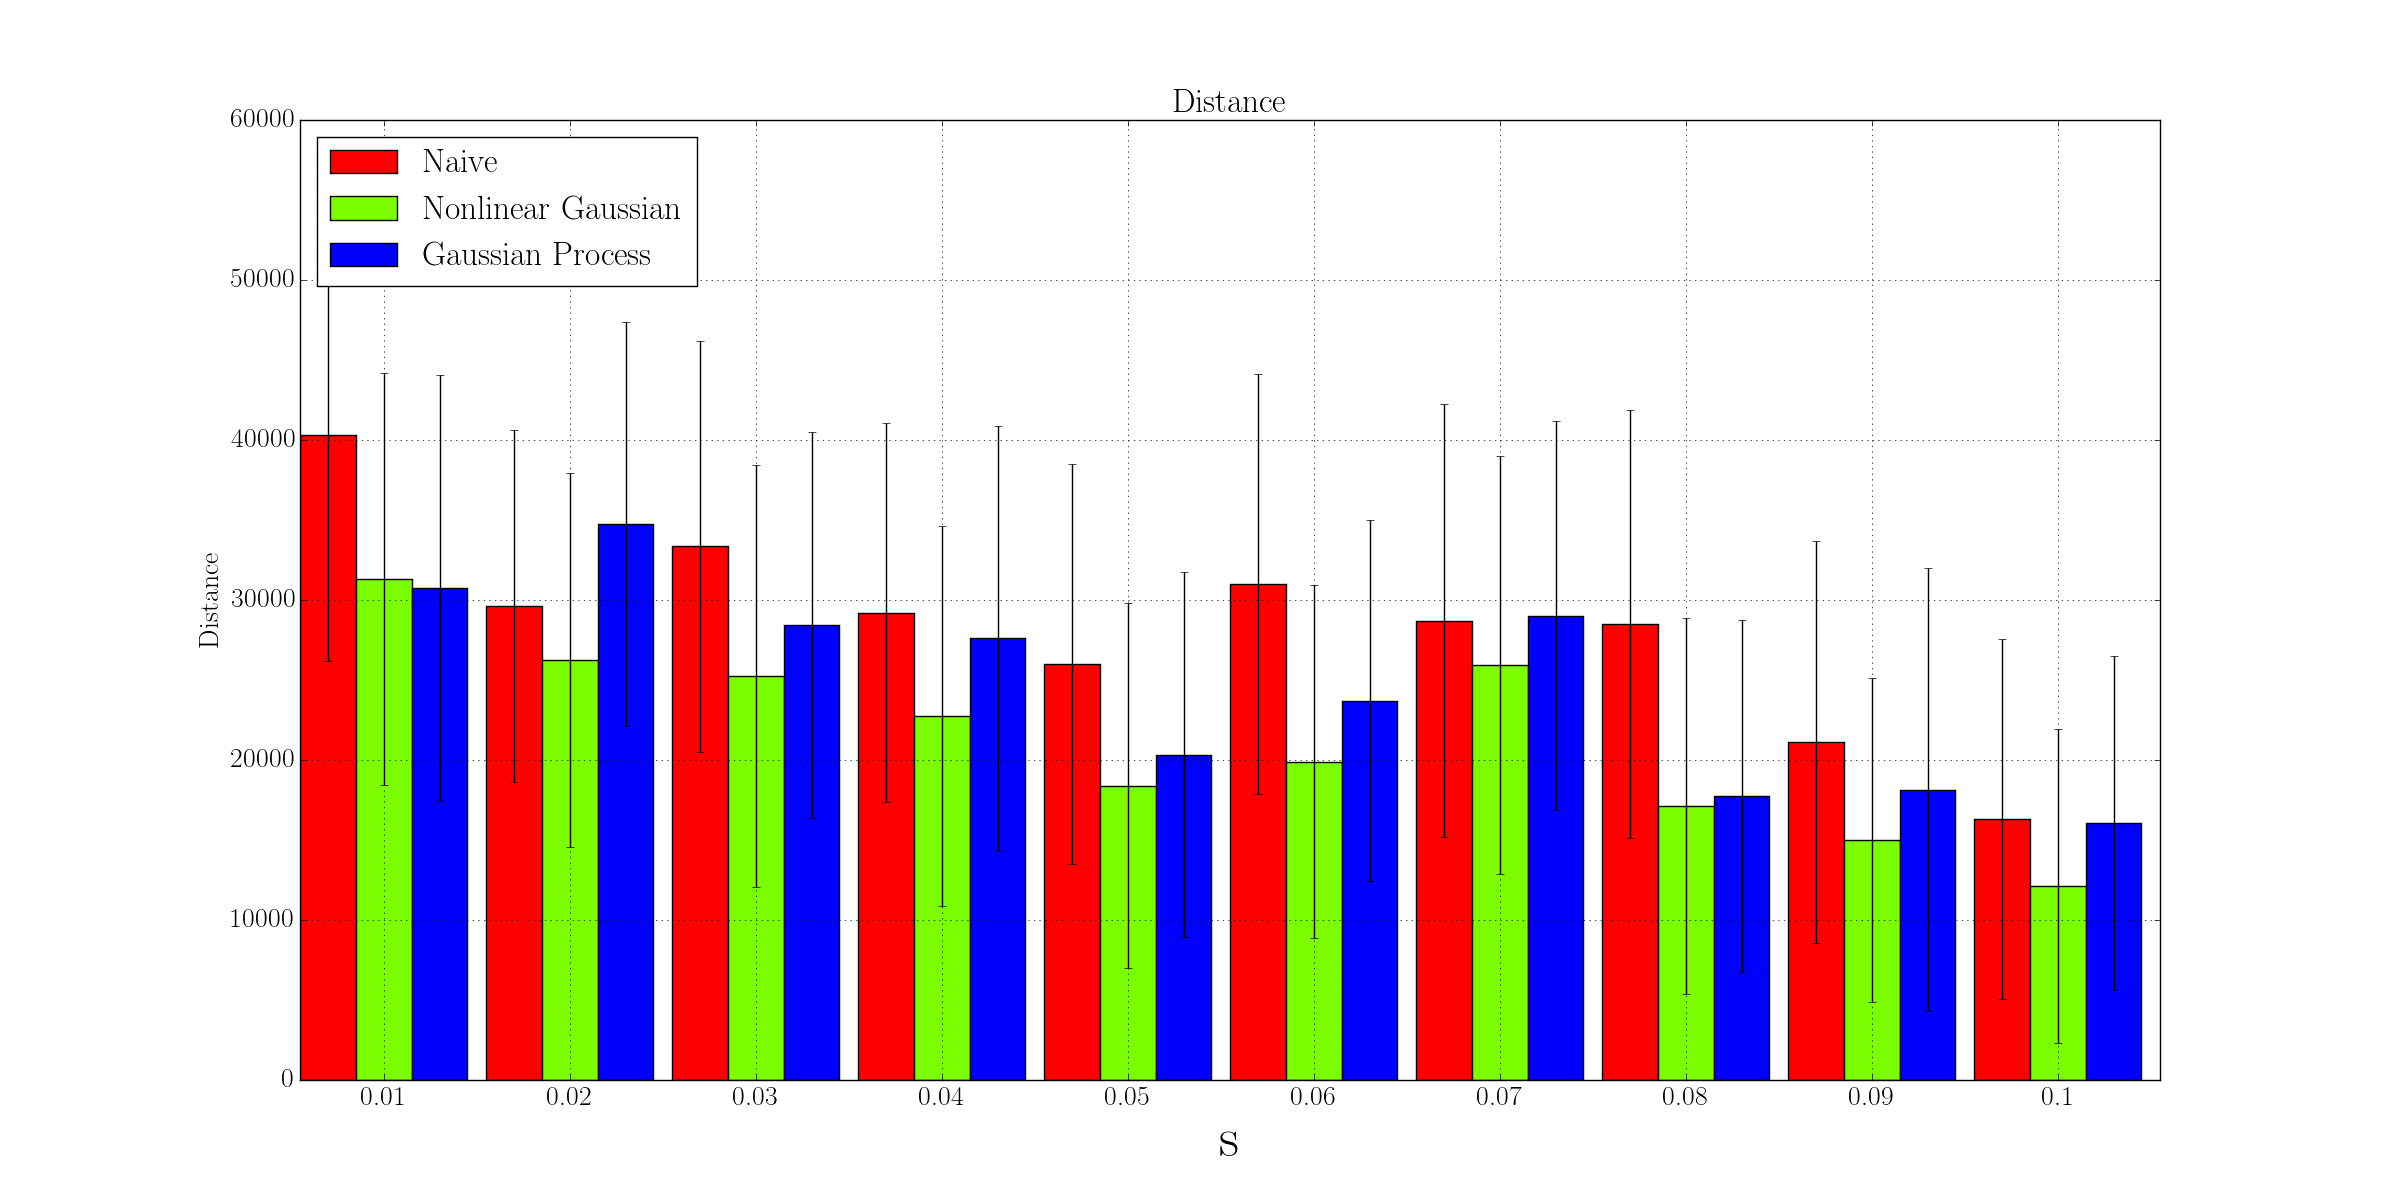
\includegraphics[width=\textwidth]{dist}
  \caption{Average distance to predicted site to the true site that is under selection.}
  \label{fig:Fig1}
\end{figure}

\paragraph{Rank}
\begin{figure}[H]
  \centering
    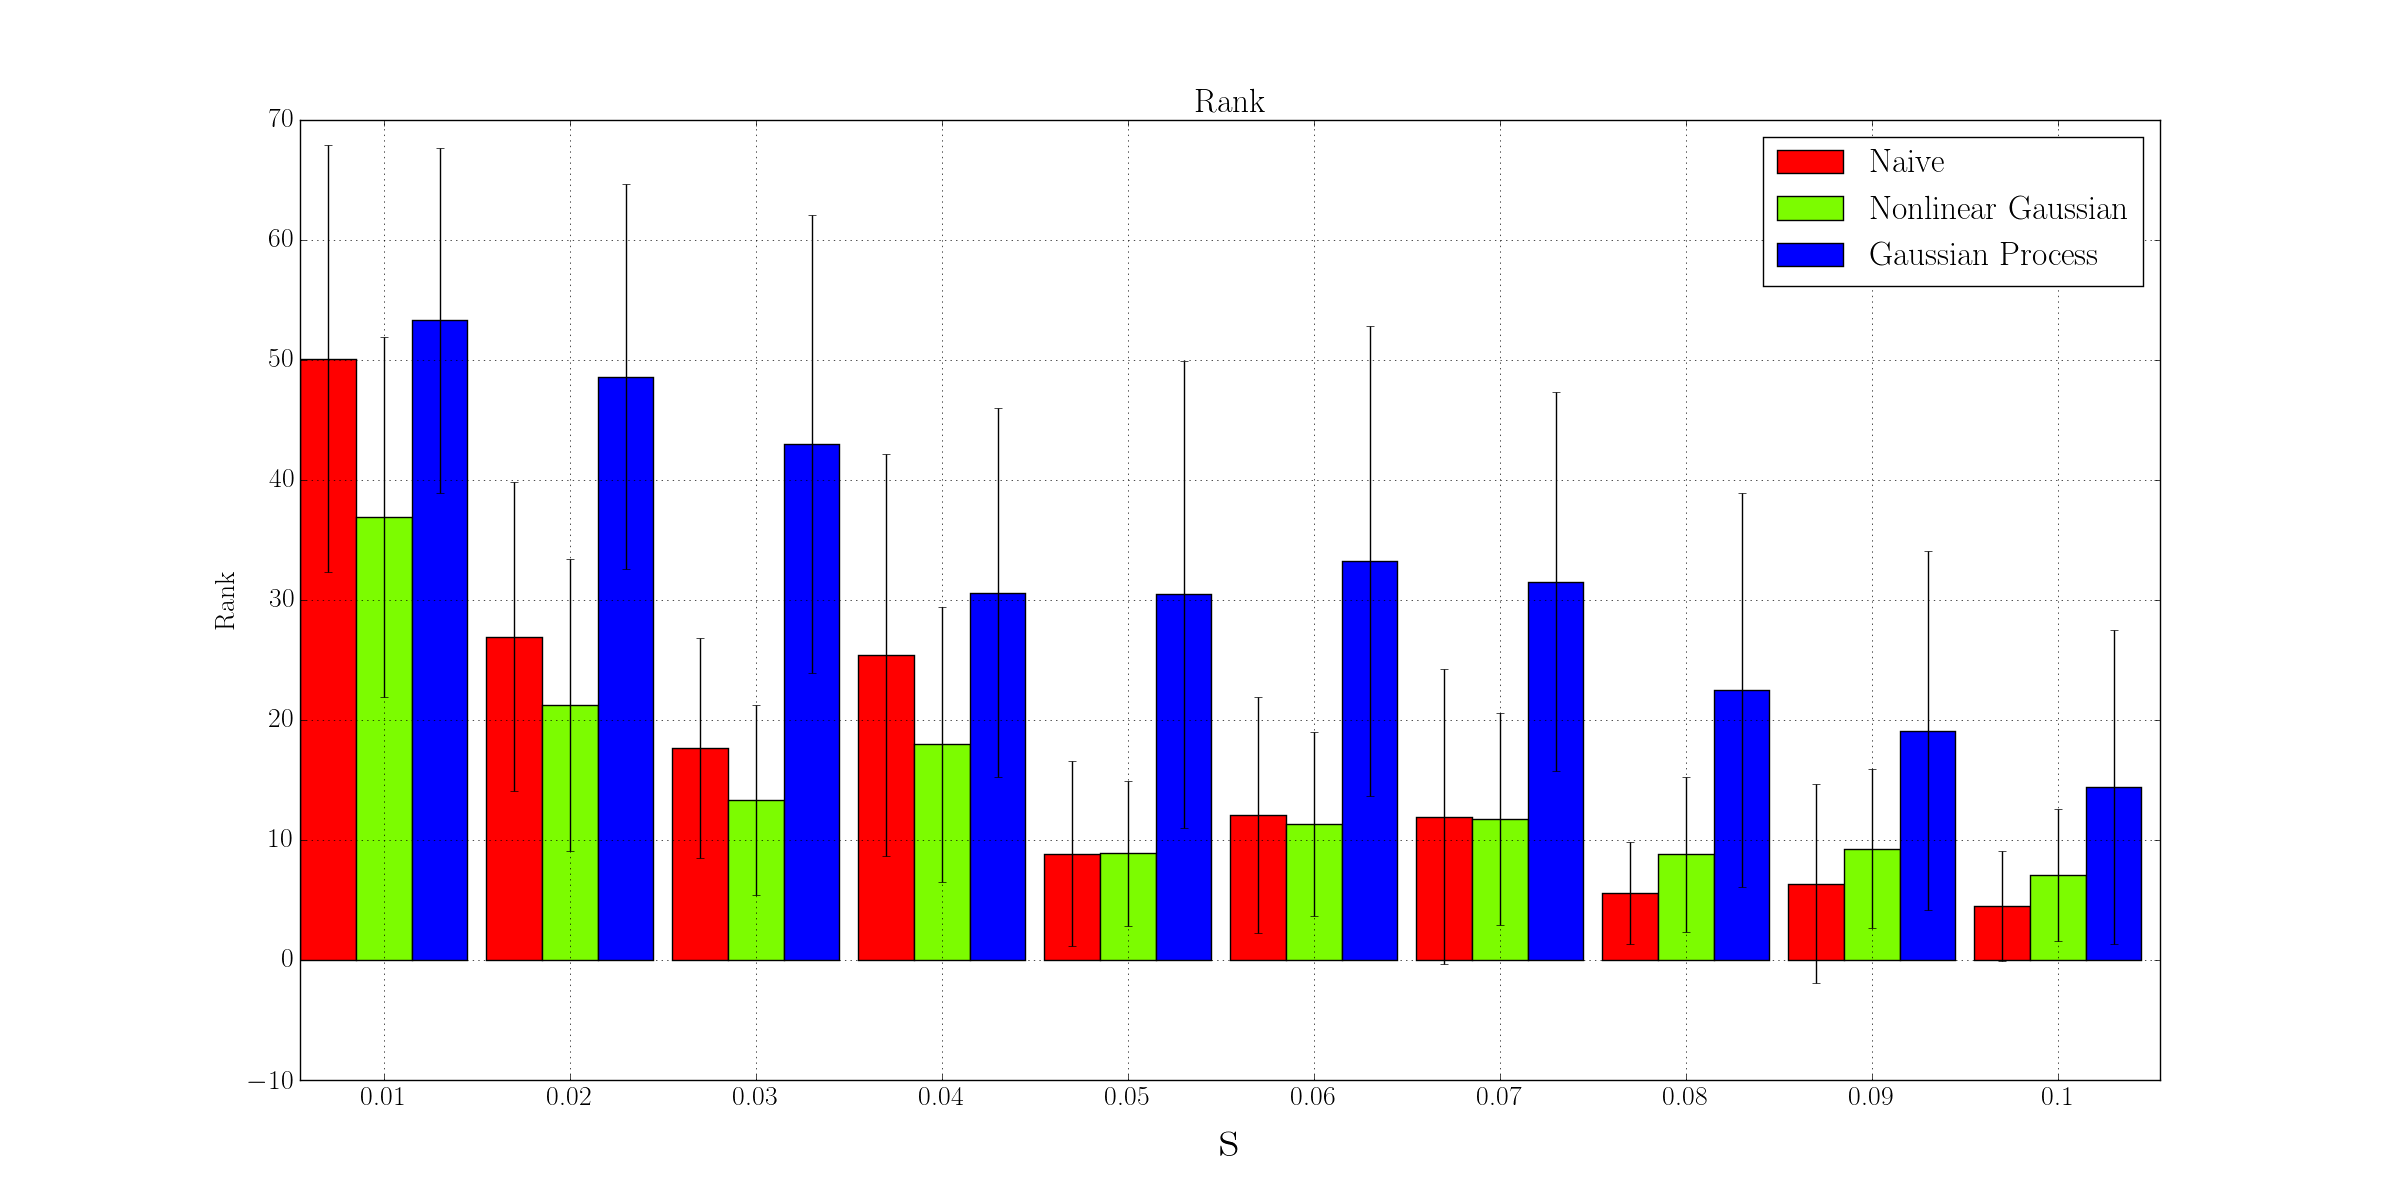
\includegraphics[width=\textwidth]{rank}
  \caption{Rank}
  \label{fig:Fig3}
\end{figure}

\paragraph{Mean Reciprocal Rank(MRR)}
\begin{figure}[H]
  \centering
    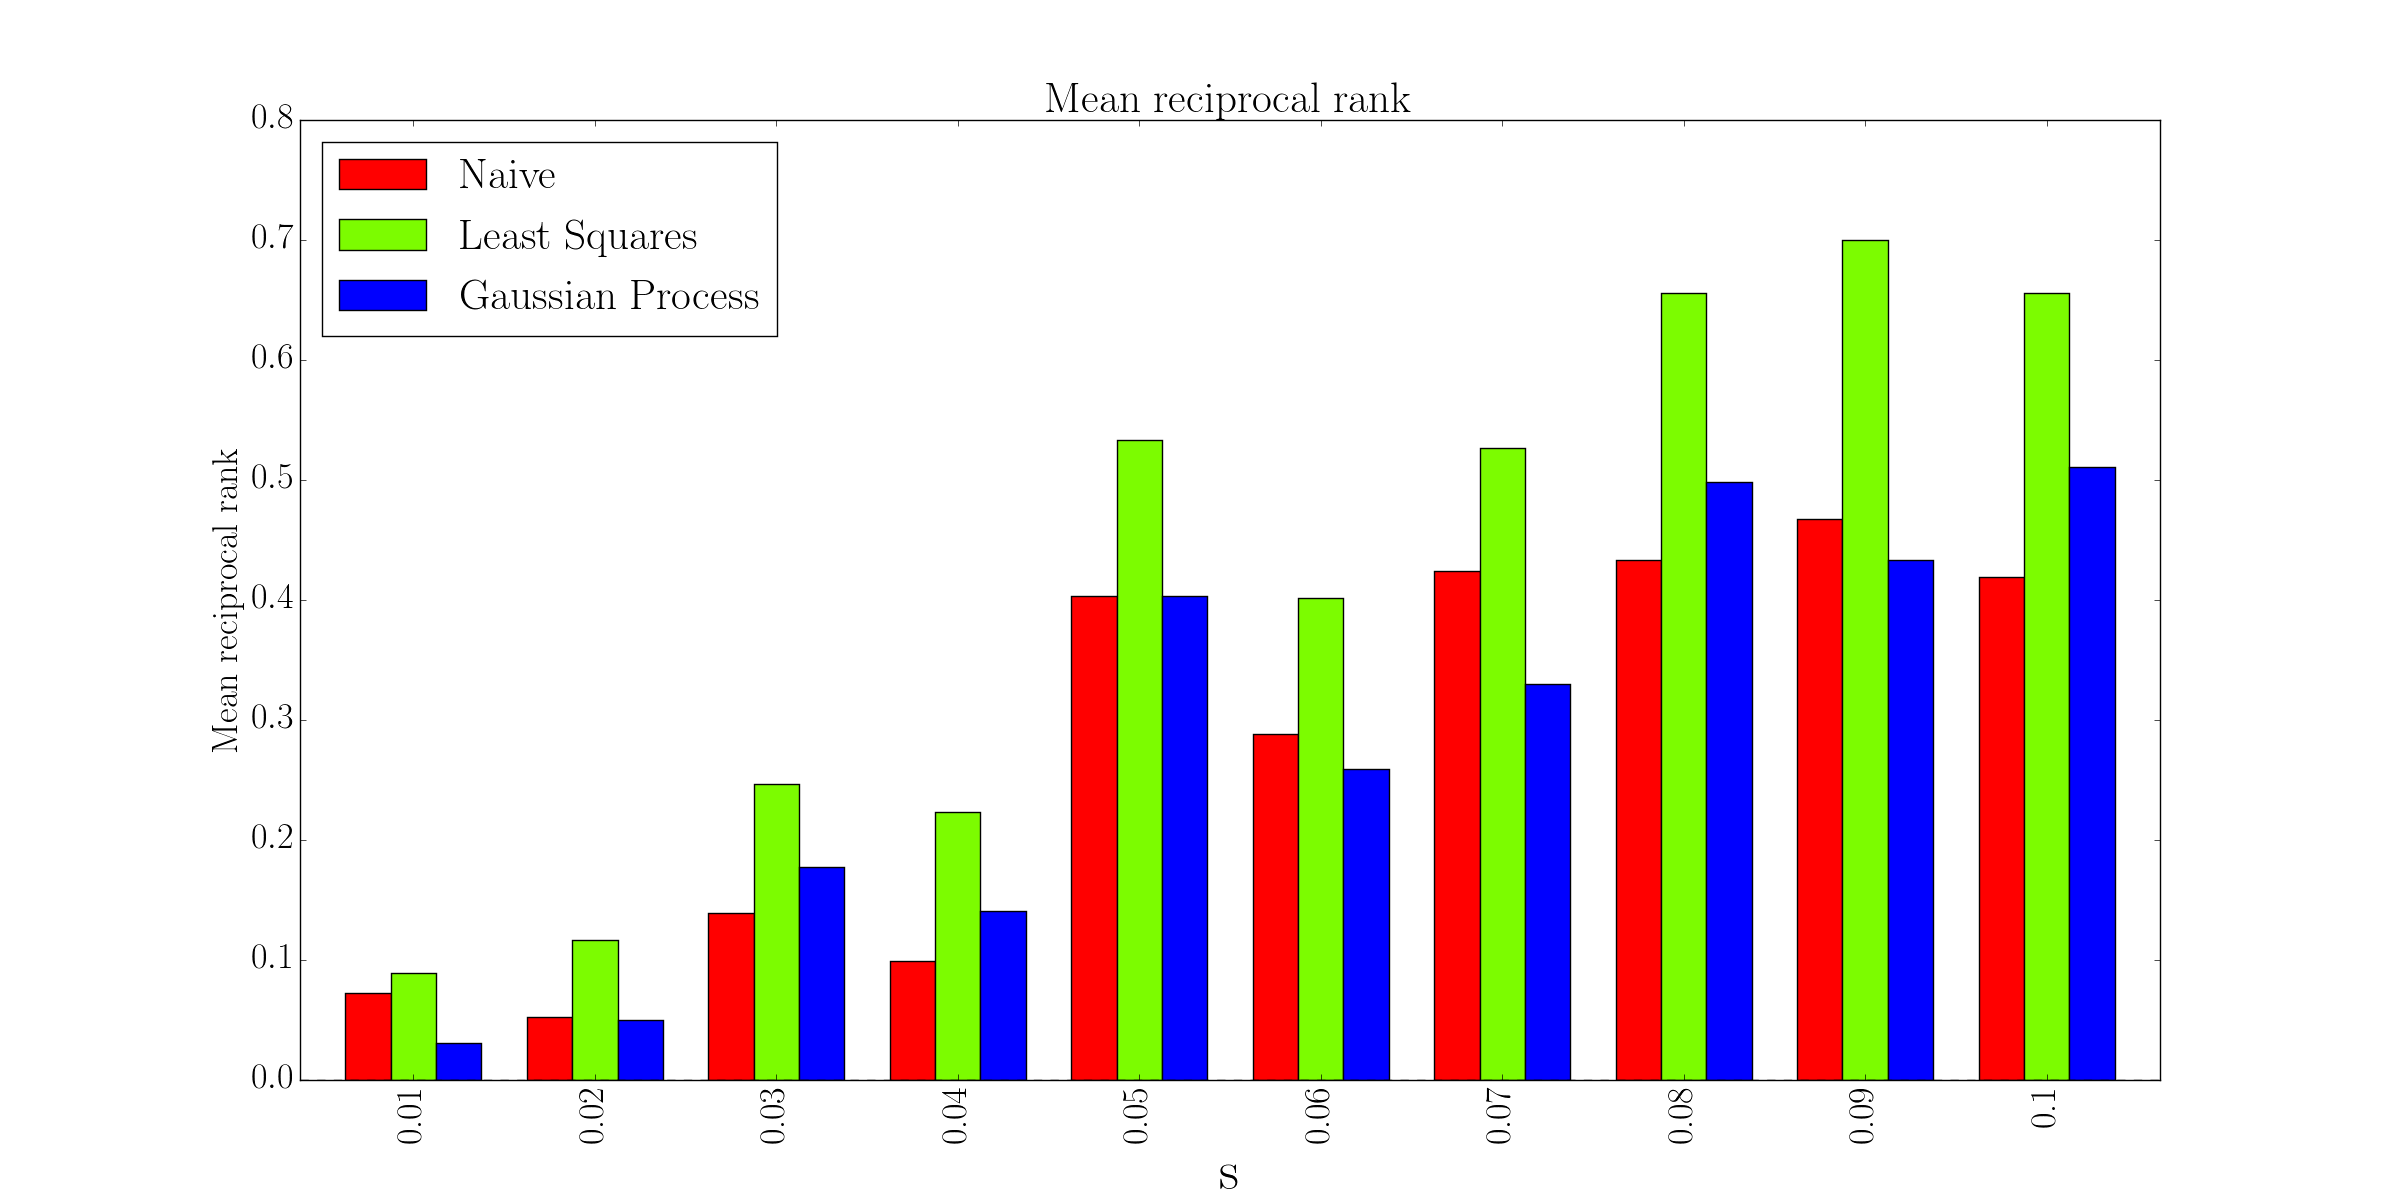
\includegraphics[width=\textwidth]{mrr}
  \caption{Mean Reciprocal}
  \label{fig:Fig2}
\end{figure}


\paragraph{Mean Average Precision (MAP)}
\begin{figure}[hh]
  \centering
    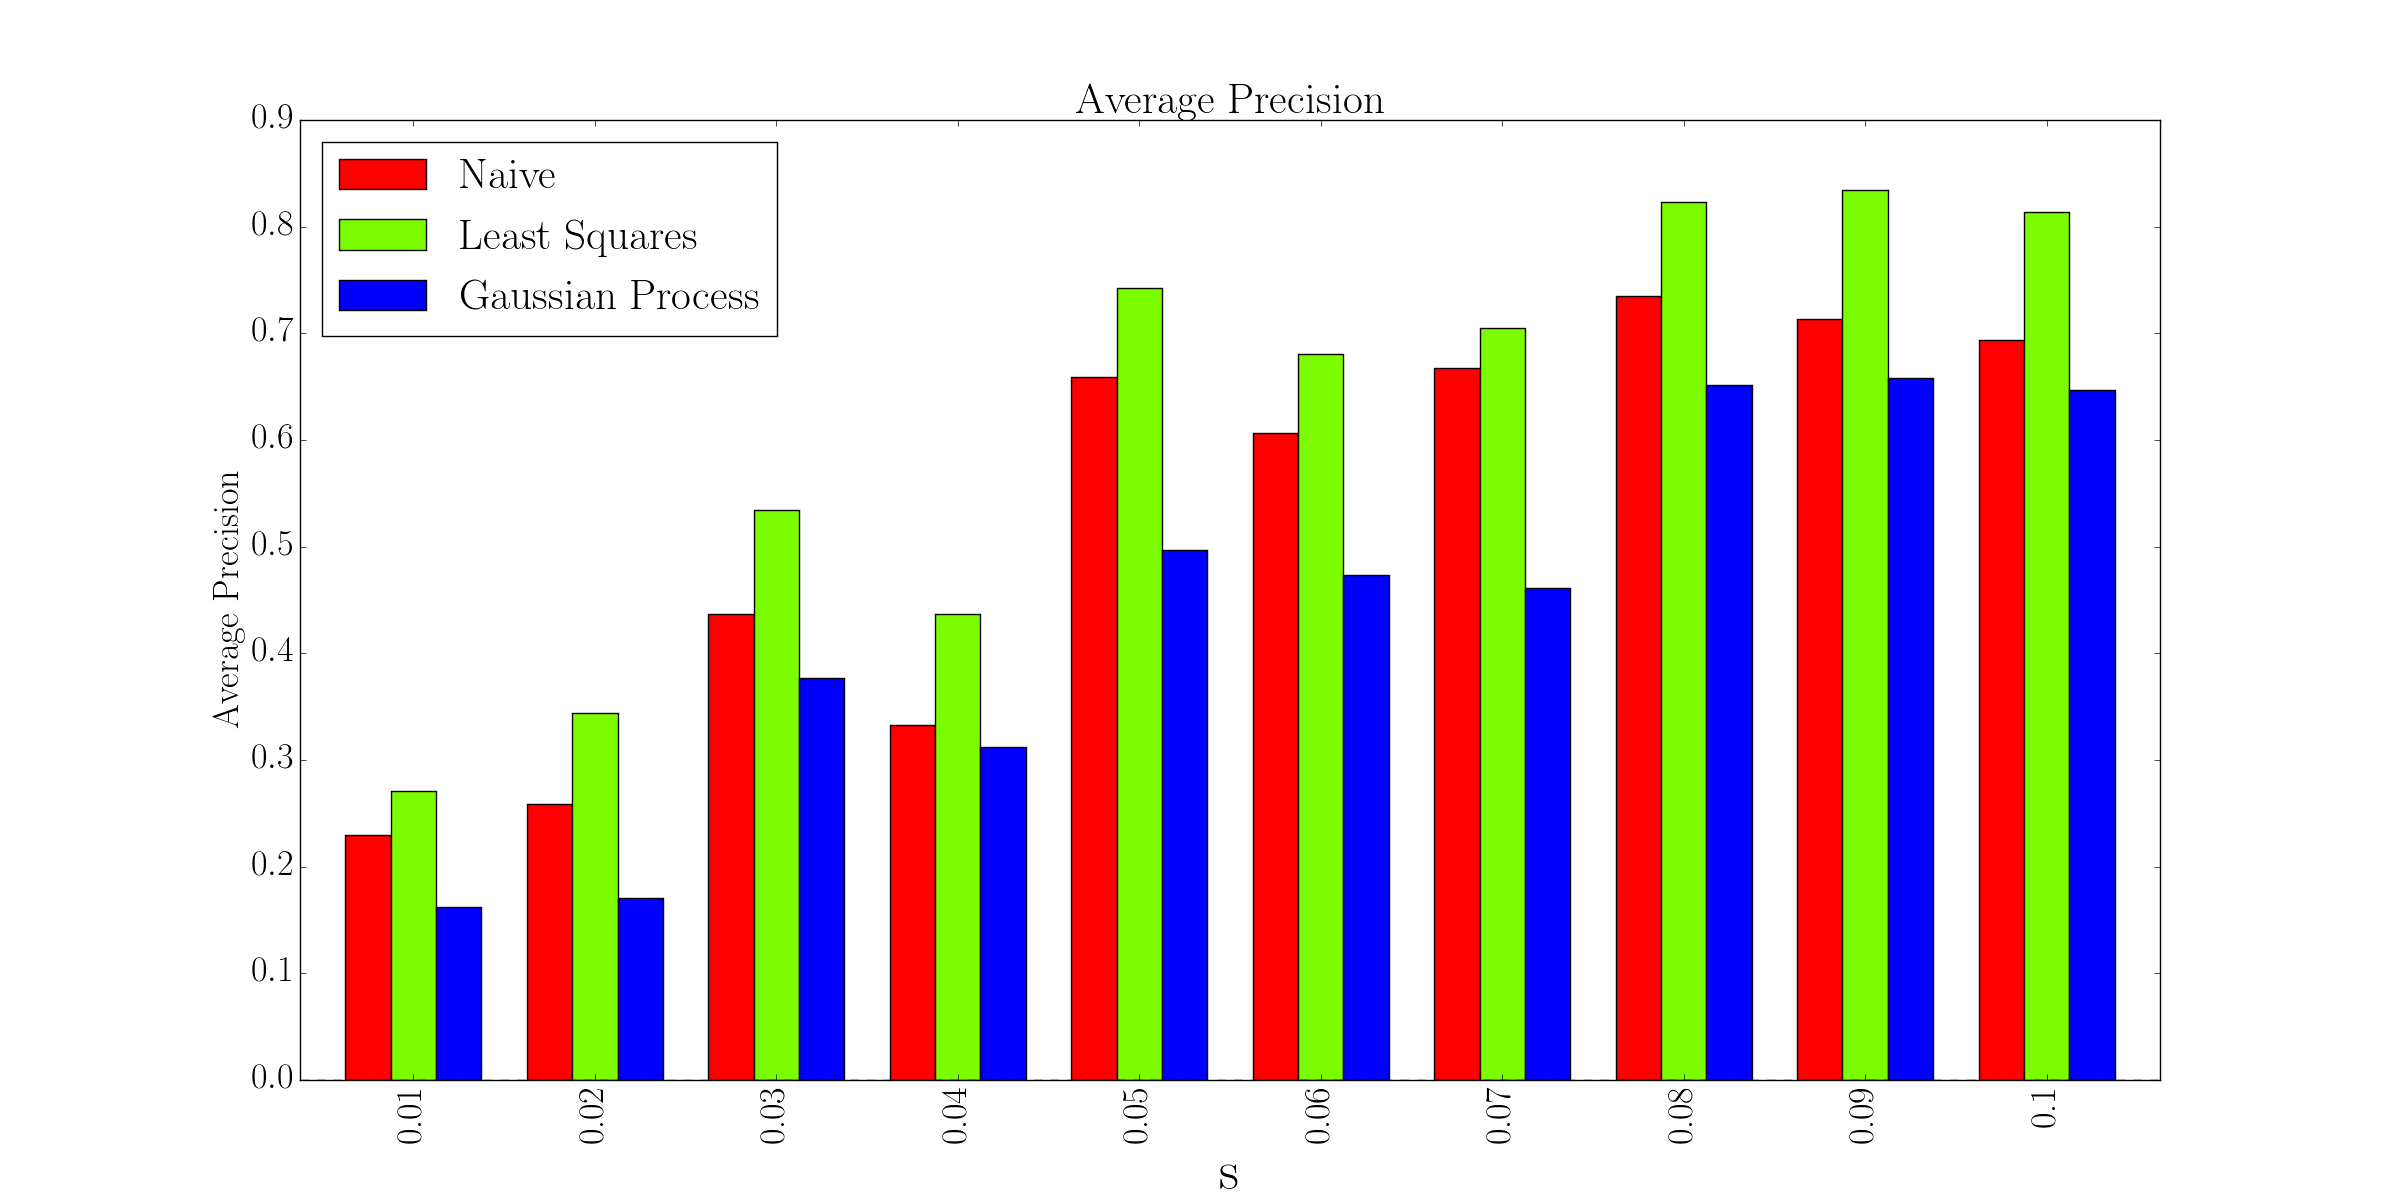
\includegraphics[width=\textwidth]{ap}
  \caption{Mean Average Precision (MAP)}
  \label{fig:Fig5}
\end{figure}


\subsubsection{Estimating Strength of Selection}
\begin{figure}[H]
  \centering
    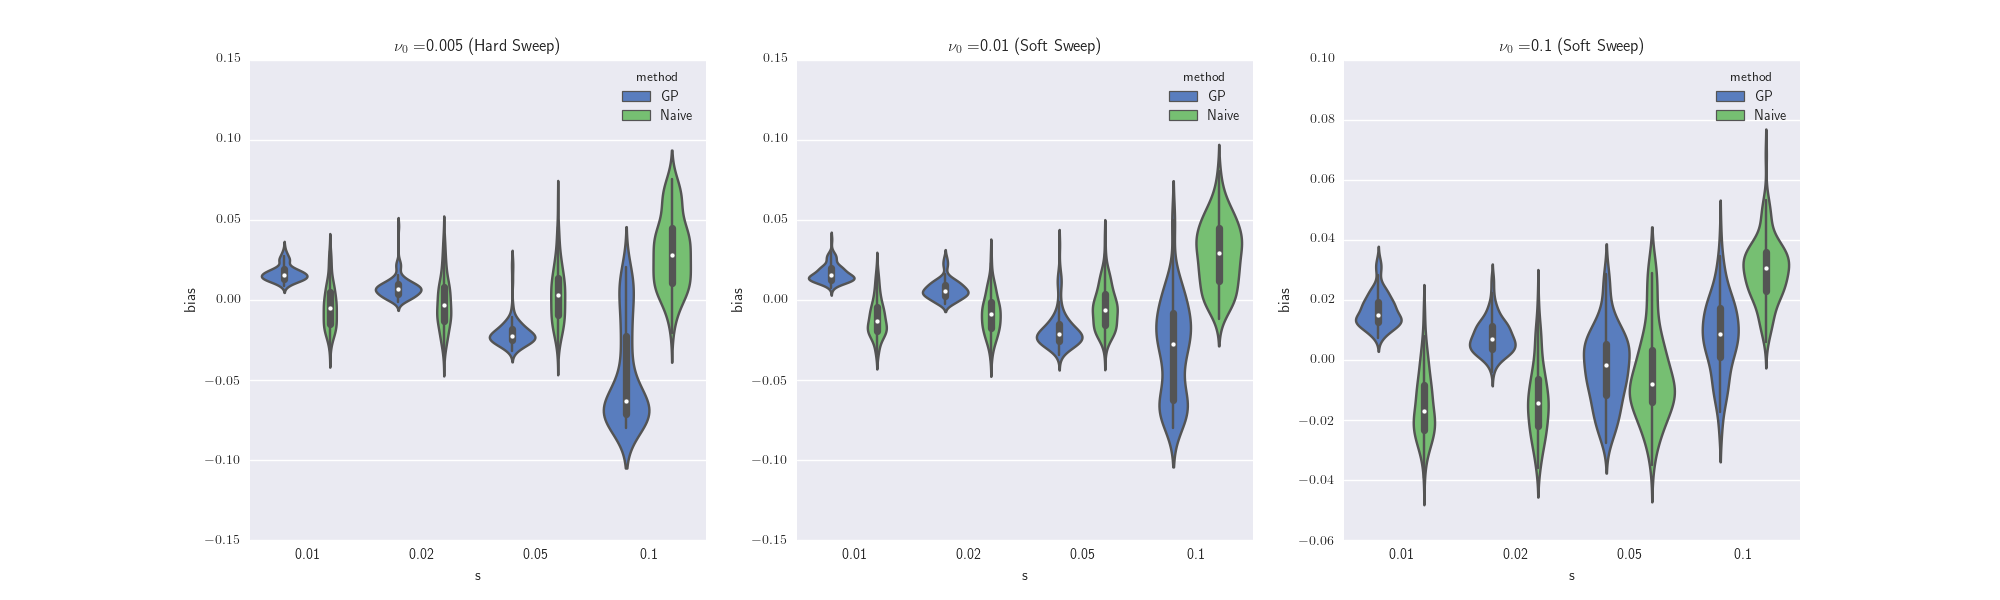
\includegraphics[width=\textwidth]{bias}
  \caption{Bias}
  \label{fig:Fig4}
\end{figure}

\subsection{Computational Performance}